\documentclass[tikz, border=10pt]{standalone}
\usepackage{tikz}

\begin{document}

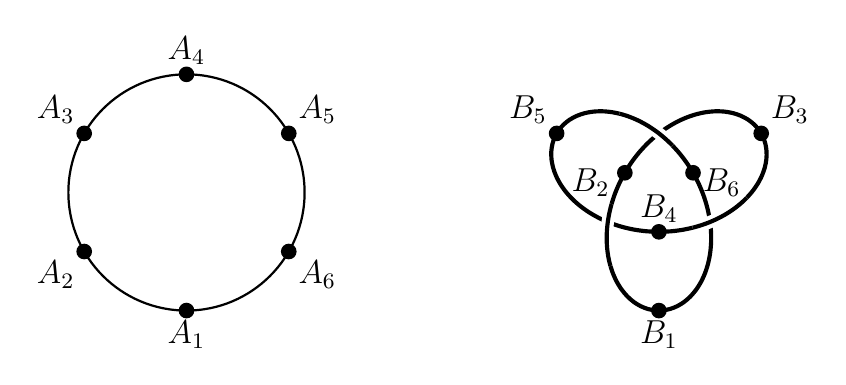
\begin{tikzpicture}[
    scale=1.0,
    every node/.style={font=\large, text=black},
    dot/.style={circle, fill=black, inner sep=2pt}
]

    % ==========================
    % LEFT FIGURE: The Circle
    % ==========================
    \begin{scope}[xshift=0cm]
        \draw[thick, black] (0,0) circle (1.5cm);

        % Brace the position values to prevent 'unknown key' error
        \foreach \i/\angle/\pos in {
            1/270/below, 
            2/210/{below left}, 
            3/150/{above left}, 
            4/90/above, 
            5/30/{above right}, 
            6/-30/{below right}} 
        {
            \node[dot] (A\i) at (\angle:1.5cm) {};
            \node[\pos] at (A\i) {$A_{\i}$};
        }
    \end{scope}


    % ==========================
    % RIGHT FIGURE: The Trefoil Knot
    % ==========================
    \begin{scope}[xshift=6cm, scale=0.5] 
        
        % NOTE: Removed the negative sign from Y coordinate to flip the shape
        % vertically so it points DOWN (matching your B1 at bottom sketch).
        
        % 1. Draw the FULL knot (Background)
        \draw[line width=1.5pt, color=black] plot[domain=0:360, samples=100, smooth] 
            ({-(sin(\x) + 2*sin(2*\x))}, {(cos(\x) - 2*cos(2*\x))});

        % 2. Draw "Over" segments (Halo Effect)
        
        % Crossing 1 (Bottom Right area in this orientation)
        \draw[line width=4.5pt, color=white] plot[domain=90:110, samples=20, smooth] 
             ({-(sin(\x) + 2*sin(2*\x))}, {(cos(\x) - 2*cos(2*\x))});
        \draw[line width=1.5pt, color=black] plot[domain=90:110, samples=20, smooth] 
             ({-(sin(\x) + 2*sin(2*\x))}, {(cos(\x) - 2*cos(2*\x))});

        % Crossing 2 (Top Center area)
        \draw[line width=4.5pt, color=white] plot[domain=210:230, samples=20, smooth] 
             ({-(sin(\x) + 2*sin(2*\x))}, {(cos(\x) - 2*cos(2*\x))});
        \draw[line width=1.5pt, color=black] plot[domain=210:230, samples=20, smooth] 
             ({-(sin(\x) + 2*sin(2*\x))}, {(cos(\x) - 2*cos(2*\x))});

        % Crossing 3 (Bottom Left area)
        \draw[line width=4.5pt, color=white] plot[domain=330:350, samples=20, smooth] 
             ({-(sin(\x) + 2*sin(2*\x))}, {(cos(\x) - 2*cos(2*\x))});
        \draw[line width=1.5pt, color=black] plot[domain=330:350, samples=20, smooth] 
             ({-(sin(\x) + 2*sin(2*\x))}, {(cos(\x) - 2*cos(2*\x))});

        % 3. Place Labels B1...B6
        % Adjusted angles for the flipped (Point Down) orientation
        \foreach \i/\t/\pos in {
            1/180/below,        
            2/240/{below left, yshift=5pt, xshift=-2pt}, 
            3/300/{above right, yshift=0pt}, 
            4/0/above,          
            5/60/{above left, yshift=0pt}, 
            6/120/{below right, yshift=5pt}} 
        {
            % Calculate coordinate
            \pgfmathsetmacro{\px}{-(sin(\t) + 2*sin(2*\t))}
            \pgfmathsetmacro{\py}{(cos(\t) - 2*cos(2*\t))} % Removed minus here too
            
            \node[dot] (B\i) at (\px,\py) {};
            \expandafter\node\expandafter[\pos] at (B\i) {$B_{\i}$};
        }
        
    \end{scope}

\end{tikzpicture}

\end{document}